\chapter{Implementacija i korisničko sučelje}
		
		
		\section{Korištene tehnologije i alati}
		
%			\textbf{\textit{dio 2. revizije}}
%			
%			 \textit{Detaljno navesti sve tehnologije i alate koji su primijenjeni pri izradi dokumentacije i aplikacije. Ukratko ih opisati, te navesti njihovo značenje i mjesto primjene. Za svaki navedeni alat i tehnologiju je potrebno \textbf{navesti internet poveznicu} gdje se mogu preuzeti ili više saznati o njima}.
			
			Komunikacija u time realizirana je korištenjem aplikacije \underline{Slack}\footnote{\url{https://slack.com/}}. Za izradu UML dijagrama korišten je alat \underline{Astah Professional}\footnote{\url{http://astah.net/editions/professional}}, a za sustav za upravljanje izvornim kodom korišten je \underline{Git}\footnote{\url{https://git-scm.com/}}. Udaljeni repozitorij projekta je dostupan na web platformi \underline{Gitlab}\footnote{\url{https://gitlab.com/}}.
			
			Kao razvojno okruženje korišten je \underline{Eclipse}\footnote{\url{https://www.eclipse.org/}} - integrirano razvojno okruženje (IDE) tvrtke Eclipse Foundation. Služi prventstveno za razvoj aplikacija u Javi, ali aplikacije se mogu raditi i u drugim programskim jezicima pomoću plug-ina.
			
			Aplikacija je napisana koristeći radni okvir \underline{Spring Boot}\footnote{\url{https://spring.io/projects/spring-boot}} i jezik \underline{Java}\footnote{\url{https://www.java.com/en/}} za izradu backenda te \underline{React}\footnote{\url{https://reactjs.org/}} i jezik \underline{JavaScript}\footnote{\url{https://www.javascript.com/}} za izradu frontenda. React je biblioteka u JavaScriptu za izgradnju korisničkih sučelja. React posjeduje tvrtka Facebook koja ga također i održava. React se najčešće koristi kao osnova u razvoju web ili mobilnih aplikacija. Radni okvir Spring Boot ima mikro servis arhitekturu koja omogućuje da svaki servis ima svoj vlastiti proces što je vrlo korisno pri razvoju aplikacija.
			
			Baza podataka nalazi se na poslužitelju u oblaku \underline{Heroku}\footnote{\url{https://www.heroku.com/}}
			
			\eject 

		
	
		\section{Ispitivanje programskog rješenja}
			
%			\textbf{\textit{dio 2. revizije}}\\
%			
%			 \textit{U ovom poglavlju je potrebno opisati provedbu ispitivanja implementiranih funkcionalnosti na razini komponenti i na razini cijelog sustava s prikazom odabranih ispitnih slučajeva. Studenti trebaju ispitati temeljnu funkcionalnost i rubne uvjete.}
	
			\clearpage
			\subsection{Ispitivanje komponenti}
%			\textit{Potrebno je provesti ispitivanje jedinica (engl. unit testing) nad razredima koji implementiraju temeljne funkcionalnosti. Razraditi \textbf{minimalno 6 ispitnih slučajeva} u kojima će se ispitati redovni slučajevi, rubni uvjeti te izazivanje pogreške (engl. exception throwing). Poželjno je stvoriti i ispitni slučaj koji koristi funkcionalnosti koje nisu implementirane. Potrebno je priložiti izvorni kôd svih ispitnih slučajeva te prikaz rezultata izvođenja ispita u razvojnom okruženju (prolaz/pad ispita). }
			\newcounter{testcase}
			\refstepcounter{testcase}
			
			Ispitivanje komponenti \engl{unit testing} se kontinuirano prati koristeći GitLab CI/CD\footnote{\url{https://docs.gitlab.com/ee/ci/}}. 
			U nastavku su prikazani ispitni slučajevi komponenti koji se prate, njihovi očekivani i trenutni rezultati, a na kraju potpoglavlja je prikazan rezultatizvođenja ispita u razvojnom okruženju.  \\
			
			\noindent \textbf{Ispitni slučaj \thetestcase: Registracija korisnika sprema korisnika u bazu podataka} \\
			\noindent \textbf{Ulaz:}
			\begin{packed_enum}
				\item Pozivanje metode za registraciju korisnika s ispravnim podacima.
			\end{packed_enum}
			\noindent \textbf{Očekivani rezultat:}
			\begin{packed_enum}
				\item[1.a] Korisnik je spremljen u bazu podataka.
			\end{packed_enum}
			\noindent \textbf{Izvorni kod:}
			\begin{listing}[H]
\begin{minted}{java}
@Test
void testRegistrationSavesUser() {
    UserDTO firstUser = new UserDTO("username", "email@email.com", "password");

    userController.signUp(firstUser);

    // User was saved
    verify(userRepository, times(1))
            .save(any());
}
\end{minted}
				\caption{Izvorni kod za ispitni slučaj \thetestcase}
				\label{unittestcase1}
			\end{listing}
			\noindent \textbf{Rezultat:} Očekivani rezultat je zadovoljen. Registracija korisnika s ispravnim podacima je uspješno spremila tog korisnika u bazu podataka. 
			\refstepcounter{testcase}
			\clearpage

			\noindent \textbf{Ispitni slučaj \thetestcase: Registracija dva korisnika s istom e-mail adresom} \\
			\noindent \textbf{Ulaz:}
			\begin{packed_enum}
				\item Pozivanje metode za registraciju korisnika.
				\item Pozivanje metode za registraciju korisnika s istom e-mail adresom.
			\end{packed_enum}
			\noindent \textbf{Očekivani rezultat:}
			\begin{packed_enum}
				\item[1.a] Korisnik je spremljen u bazu podataka.
				\item[2.a] Izazvana je iznimka zbog duplicirane e-mail adrese.
			\end{packed_enum}
			\noindent \textbf{Izvorni kod:}
			\begin{listing}[H]
\begin{minted}{java}
@Test
void testRegistrationWithDuplicateEmailAddress() {
	UserDTO firstUser = new UserDTO("username1", "email@email.com"
                                         "password1");
	UserDTO secondUser = new UserDTO("username2", "email@email.com",
                                         "password2");
		
	userController.signUp(firstUser);
	
	// First user was saved
	verify(userRepository, times(1))
	    .save(any());
	
	// Second user causes an exception
	assertThrows(Exception.class, () -> userController.signUp(secondUser));
}
\end{minted}
				\caption{Izvorni kod za ispitni slučaj \thetestcase}
				\label{testRegistrationWithDuplicateEmailAddress}
			\end{listing}
			\noindent \textbf{Rezultat:} Očekivani rezultat je zadovoljen. Registracija prvog korisnika uspješno sprema tog korisnika u bazu podataka, dok registracija drugog korisnika rezultira iznimkom. 
			\refstepcounter{testcase}
			\clearpage

			\noindent \textbf{Ispitni slučaj \thetestcase: Registracija dva korisnika s istim korisničkim imenom} \\
			\noindent \textbf{Ulaz:}
			\begin{packed_enum}
				\item Pozivanje metode za registraciju korisnika.
				\item Pozivanje metode za registraciju korisnika s istim korisničkim imenom.
			\end{packed_enum}
			\noindent \textbf{Očekivani rezultat:}
			\begin{packed_enum}
				\item[1.a] Korisnik je spremljen u bazu podataka.
				\item[2.a] Izazvana je iznimka zbog dupliciranog korisničkog imena.
			\end{packed_enum}
			\noindent \textbf{Izvorni kod:}
			\begin{listing}[H]
\begin{minted}{java}
@Test
void testRegistrationWithDuplicateUsername() {
	UserDTO firstUser = new UserDTO("username", "email1@email.com"
                                         "password1");
	UserDTO secondUser = new UserDTO("username", "email2@email.com",
                                         "password2");
		
	userController.signUp(firstUser);
	
	// First user was saved
	verify(userRepository, times(1))
	    .save(any());
	
	// Second user causes an exception
	assertThrows(Exception.class, () -> userController.signUp(secondUser));
}
\end{minted}
				\caption{Izvorni kod za ispitni slučaj \thetestcase}
				\label{test5}
			\end{listing}
			\noindent \textbf{Rezultat:} Očekivani rezultat je zadovoljen. Registracija prvog korisnika uspješno sprema tog korisnika u bazu podataka, dok registracija drugog korisnika rezultira iznimkom. 
			\refstepcounter{testcase}
			\clearpage
			
			\noindent \textbf{Ispitni slučaj \thetestcase: Korisnik smije dohvatiti vlastite osobne podatke} \\
			\noindent \textbf{Ulaz:}
			\begin{packed_enum}
				\item Pozivanje metode za dohvat osobnih podataka za trenutno prijavljenog korisnika.
			\end{packed_enum}
			\noindent \textbf{Očekivani rezultat:}
			\begin{packed_enum}
				\item[1.a] Vraćeni su osobni podaci prijavljenog korisnika.
			\end{packed_enum}
			\noindent \textbf{Izvorni kod:}

			\begin{listing}[H]
\begin{minted}{java}
@Test
void testUserCanFetchItsOwnData() {
    userController.getUserInformation("logged_in_user",
            () -> "logged_in_user");

    // Verify interaction with database
    verify(userRepository, times(1))
            .findByUsername(anyString());
}
\end{minted}
				\caption{Izvorni kod za ispitni slučaj \thetestcase}
				\label{test2}
			\end{listing}
			\noindent \textbf{Rezultat:} Očekivani rezultat je zadovoljen. Dohvaćeni su osobni podaci prijavljenog korisnika.
			\refstepcounter{testcase}
			\clearpage

			\noindent \textbf{Ispitni slučaj \thetestcase: Korisnik ne smije moći dohvatiti osobne podatke drugog korisnika} \\
			\noindent \textbf{Ulaz:}
			\begin{packed_enum}
				\item Pozivanje metode za dohvat osobnih podataka za korisnika koji nije trenutno prijavljen.
			\end{packed_enum}
			\noindent \textbf{Očekivani rezultat:}
			\begin{packed_enum}
				\item[1.a] Izazvana je iznimka zbog pokušaja dohvata tuđih podataka.
			\end{packed_enum}
			\noindent \textbf{Izvorni kod:}

			\begin{listing}[H]
\begin{minted}{java}
@Test
void testUserCannotFetchOthersData() {
    assertThrows(Exception.class, () ->
            userController.getUserInformation("different_user", 
                    () -> "logged_in_user"));

    // Verify no interaction with database
    verify(userRepository, times(0))
            .findByUsername(anyString());
}
\end{minted}
				\caption{Izvorni kod za ispitni slučaj \thetestcase}
				\label{test2}
			\end{listing}
			\noindent \textbf{Rezultat:} Očekivani rezultat je zadovoljen. Izazvana je iznimka pri pokušaju dohvata osobnih podataka drugog korisnika.
			\refstepcounter{testcase}
			\clearpage

			\noindent \textbf{Ispitni slučaj \thetestcase: Dohvat podataka o postojećem kontejneru} \\
			\noindent \textbf{Ulaz:}
			\begin{packed_enum}
				\item Pozivanje metode za dohvat podataka o kontejneru s valjanim identifikatorom kontejnera.
			\end{packed_enum}
			\noindent \textbf{Očekivani rezultat:}
			\begin{packed_enum}
				\item[1.a] Vraćeni su podaci o kontejneru s tim identifikatorom.
			\end{packed_enum}
			\noindent \textbf{Izvorni kod:}

			\begin{listing}[H]
\begin{minted}{java}
@Test
void testFetchingInformationAboutExistingWasteContainer() {
    wasteContainerController.findByID(EXISTING_WASTE_CONTAINER_ID);

    // Verify interaction with database
    verify(wasteContainerRepository, times(1))
            .findById(EXISTING_WASTE_CONTAINER_ID);
}
\end{minted}
				\caption{Izvorni kod za ispitni slučaj \thetestcase}
				\label{test2}
			\end{listing}
			\noindent \textbf{Rezultat:} Očekivani rezultat je zadovoljen. Dohvaćeni su podaci o kontejneru s tim identifikatorom.
			\refstepcounter{testcase}
			\clearpage
			
			\noindent \textbf{Ispitni slučaj \thetestcase: Dohvat podataka o nepostojećem kontejneru} \\
			\noindent \textbf{Ulaz:}
			\begin{packed_enum}
				\item Pozivanje metode za dohvat podataka o kontejneru s nevaljanim identifikatorom kontejnera.
			\end{packed_enum}
			\noindent \textbf{Očekivani rezultat:}
			\begin{packed_enum}
				\item[1.a] Izazvana je iznimka zbog pokušaja dohvata podataka o kontejneru koji ne postoji.
			\end{packed_enum}
			\noindent \textbf{Izvorni kod:}

			\begin{listing}[H]
\begin{minted}{java}
@Test
void testFetchingInformationAboutNonExistantWasteContainer() {
    assertThrows(Exception.class,
            () -> 
	       wasteContainerController.findByID(NON_EXISTANT_WASTE_CONTAINER_ID));

    // Verify interaction with database
    verify(wasteContainerRepository, times(1))
            .findById(NON_EXISTANT_WASTE_CONTAINER_ID);
}
\end{minted}
				\caption{Izvorni kod za ispitni slučaj \thetestcase}
				\label{test3}
			\end{listing}
			\noindent \textbf{Rezultat:} Očekivani rezultat je zadovoljen. Dohvat podataka o nepostojećem kontejneru je izazvao iznimku.
			\refstepcounter{testcase}

\begin{listing}[H]
	\begin{minted}[linenos,breaklines,fontsize=\footnotesize,frame=lines]{text}
[INFO] --- maven-surefire-plugin:2.22.2:test (default-test) @ manje-smece-vise-srece-backend ---
[INFO] 
[INFO] -------------------------------------------------------
[INFO]  T E S T S
[INFO] -------------------------------------------------------
[INFO] Running hr.fer.opp.bashcrash.manjesmecevisesrece.rest.WasteContainerControllerTest
[INFO] Tests run: 2, Failures: 0, Errors: 0, Skipped: 0, Time elapsed: 0.656 s - in hr.fer.opp.bashcrash.manjesmecevisesrece.rest.WasteContainerControllerTest
[INFO] Running hr.fer.opp.bashcrash.manjesmecevisesrece.rest.UserControllerTest
[INFO] Tests run: 5, Failures: 0, Errors: 0, Skipped: 0, Time elapsed: 0.118 s - in hr.fer.opp.bashcrash.manjesmecevisesrece.rest.UserControllerTest
[INFO] 
[INFO] Results:
[INFO] 
[INFO] Tests run: 7, Failures: 0, Errors: 0, Skipped: 0
[INFO] 
[INFO] ------------------------------------------------------------------------
[INFO] BUILD SUCCESS
[INFO] ------------------------------------------------------------------------
[INFO] Total time:  6.019 s
[INFO] Finished at: 2020-01-02T23:31:26+01:00
[INFO] ------------------------------------------------------------------------
	\end{minted}
	\caption{Prikaz rezultata izvođenja ispita u razvojnom okruženju}
\end{listing}
			
			\subsection{Ispitivanje sustava}
			
%			 \textit{Potrebno je provesti i opisati ispitivanje sustava koristeći radni okvir Selenium\footnote{\url{https://www.seleniumhq.org/}}. Razraditi \textbf{minimalno 4 ispitna slučaja} u kojima će se ispitati redovni slučajevi, rubni uvjeti te poziv funkcionalnosti koja nije implementirana/izaziva pogrešku kako bi se vidjelo na koji način sustav reagira kada nešto nije u potpunosti ostvareno. Ispitni slučaj se treba sastojati od ulaza (npr. korisničko ime i lozinka), očekivanog izlaza ili rezultata, koraka ispitivanja i dobivenog izlaza ili rezultata.\\ }
%			 
%			 \textit{Izradu ispitnih slučajeva pomoću radnog okvira Selenium moguće je provesti pomoću jednog od sljedeća dva alata:}
%			 \begin{itemize}
%			 	\item \textit{dodatak za preglednik \textbf{Selenium IDE} - snimanje korisnikovih akcija radi automatskog ponavljanja ispita	}
%			 	\item \textit{\textbf{Selenium WebDriver} - podrška za pisanje ispita u jezicima Java, C\#, PHP koristeći posebno programsko sučelje.}
%			 \end{itemize}
%		 	 \textit{Detalji o korištenju alata Selenium bit će prikazani na posebnom predavanju tijekom semestra.}
			
			\eject 
		
		
		\section{Dijagram razmještaja}
			
			% \textbf{\textit{dio 2. revizije}}
			
			 % \textit{Potrebno je umetnuti \textbf{specifikacijski} dijagram razmještaja i opisati ga. Moguće je umjesto specifikacijskog dijagrama razmještaja umetnuti dijagram razmještaja instanci, pod uvjetom da taj dijagram bolje opisuje neki važniji dio sustava.}
			
			\begin{figure} [H]
			    \centering
			    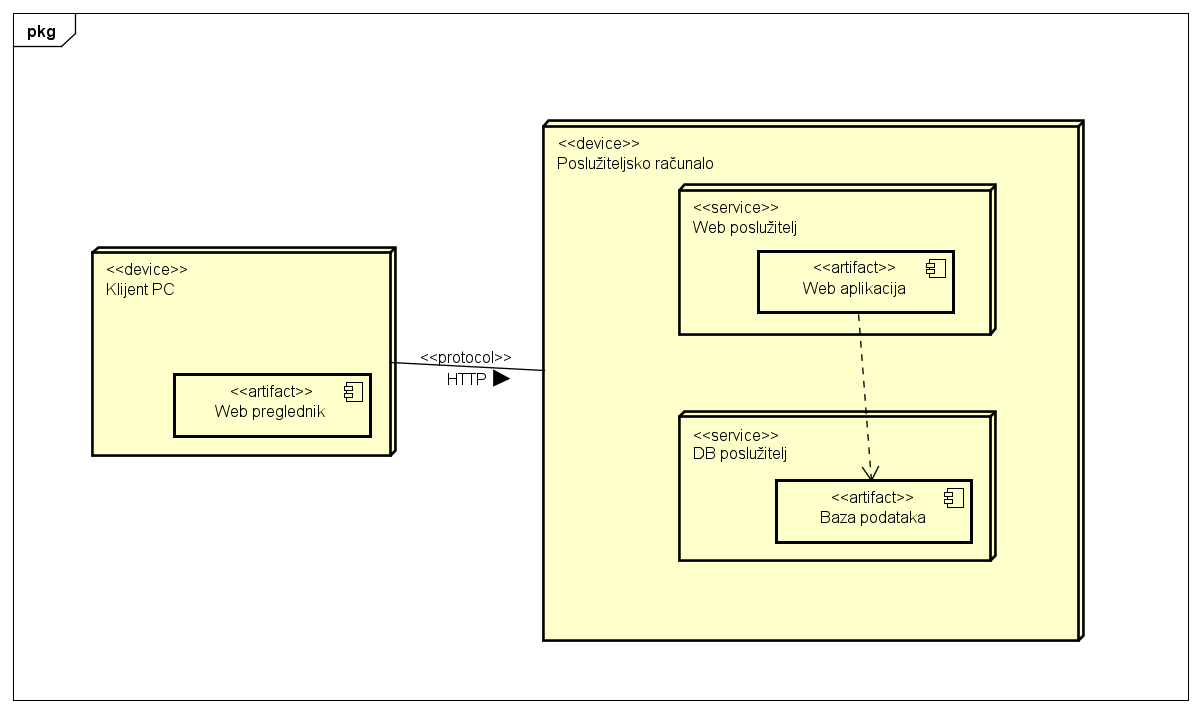
\includegraphics[width=1.0\linewidth]{slike/Deployment_Diagram.png}
	            \caption{Dijagram razmještaja}
				\label{fig:Dijagram razmještaja}
		
			\eject 
		
		\section{Upute za puštanje u pogon}
		
			% \textbf{\textit{dio 2. revizije}}\\
		
			 % \textit{U ovom poglavlju potrebno je dati upute za puštanje u pogon (engl. deployment) ostvarene aplikacije. Na primjer, za web aplikacije, opisati postupak kojim se od izvornog kôda dolazi do potpuno postavljene baze podataka i poslužitelja koji odgovara na upite korisnika. Za mobilnu aplikaciju, postupak kojim se aplikacija izgradi, te postavi na neku od trgovina. Za stolnu (engl. desktop) aplikaciju, postupak kojim se aplikacija instalira na računalo. Ukoliko mobilne i stolne aplikacije komuniciraju s poslužiteljem i/ili bazom podataka, opisati i postupak njihovog postavljanja. Pri izradi uputa preporučuje se \textbf{naglasiti korake instalacije uporabom natuknica} te koristiti što je više moguće \textbf{slike ekrana} (engl. screenshots) kako bi upute bile jasne i jednostavne za slijediti.}
			
			
			 % \textit{Dovršenu aplikaciju potrebno je pokrenuti na javno dostupnom poslužitelju. Studentima se preporuča korištenje neke od sljedećih besplatnih usluga: \href{https://aws.amazon.com/}{Amazon AWS}, \href{https://azure.microsoft.com/en-us/}{Microsoft Azure} ili \href{https://www.heroku.com/}{Heroku}. Mobilne aplikacije trebaju biti objavljene na F-Droid, Google Play ili Amazon App trgovini.}
			
			
			\eject 
